\chapter{Building Accessible and Automated Mass Cytometry Analysis Tools}
\label{03cytof}

\newpage
\section{Introduction}


As outlined in Chapter \ref{01intro}, the Thiol Organoid Barcoding \textit{in situ} (TOB\textit{is}) \acrfull{mc} platform used to analyse the \acrfull{crc} organoids is already a mature approach. The effects of both \acrfull{tme} and genotypical pertubartions in this organoid system were already explored \cite{qin_cell-type-specific_2020}, but data analysis was performed using custom and discrete scripts; encumbering consistency and reproducibility for future analyses. Furthermore, the manual process of cell state annotation added further load to the analysis.

% cygnasl
To improve upon this I have designed and developed CyGNAL (CyTOF SiGNalling AnaLysis)~\cite{ferran_cardoso_tape-labcygnal_2021}, a pipeline for \acrshort{mc} data analysis with a focus on studying \acrfull{ptm} changes across multiple conditions. CyGNAL aims to streamline and bring to non-computational scientists analyses similar to those shown in Qin \emph{et al.}~\cite{qin_cell-type-specific_2020}, with the addition of dimensionality reduction embeddings and interactive visualisations. CyGNAL was published as part of Sufi \& Qin et al. \cite{sufi_multiplexed_2021} in conjunction with an updated TOBis custom mass cytometry platform for organoids.

%class
The maturity of the platform is also reflected on the properties of the markers used in the \acrshort{mc} panels, with the most robust markers achieving highly binary and specific staining. Given the importance of cell state changes to perturbations in the epithelial organoids, either in the form of intrinsic effects such as genotype or extrinsic in the form of the \acrshort{tme} or drug treatments, an automated approach of labelling and assigning a cell state to each cell in an experiment would facilitate routine analysis of \acrshort{mc} datasets. 
I thus hypothesise that we can use a machine learning approach to, using a series of canonical cell state markers, automatically predict and label the hundreds of thousands of cells captured in an \acrshort{mc} experiment. To this end I aim to develop a \acrfull{rf} classifier. This classifier will be able to ingest \acrshort{mc} data and, using manually gated datasets with cell state labels as training data, label each of the cells with one of six possible cell states: Apoptosis, G0, G1, S-phase, G2, and M-phase. 

\section{CyGNAL: CyTOF Signalling Analysis pipeline}

Published and demoed as part of Sufi \& Qin et al. 2021, CyGNAL is a publicly available tool that is routinely used to analyse \acrshort{mc} datasets both at my group and by external collaborators \cite{michelozzi_activation_2023}.

Details on the implementation, code structure and deployment can be found in Chapter \ref{02methods}. Furthermore, a step-by-step walk-through of the main CyGNAL steps is detailed in Sufi \& Qin et al. \cite{sufi_multiplexed_2021}.

In this section I will present an overview of the tool and will discuss the relevance of the different scoring systems with regards to \acrshort{mc} data in general and \acrshort{ptm} signalling panels in specific. Example outputs from CyGNAL will also be shown, both for non-interactive sections (scores and UMAP embedding) and how they can be further analysed, but also with screenshots of the interactive apps that constitute CyGNAL's visualisation steps.

\subsection{Overview and Capabilities}
% \subsection{}{Pipeline modules}

CyGNAL is a collection of scripts written mainly in Python and R. These scripts have been built around a unified code base of shared functions and a particular directory structure to facilitate interoperability between the different steps. 
Within CyGNAL's code directory, the \texttt{utils} folder has optional steps that either complement the main ones or containa aditional utilities for \acrshort{mc} data handling. 

Distribution of CyGNAL is accomplished as a container hosted in Docker Hub (\href{https://hub.docker.com/repository/docker/ferranc96/cygnal}{hub.docker.com/repository/docker/ferranc96/cygnal}). CyGNAL can also be used by downloading the project's public repository (from \href{github.com/TAPE-Lab/CyGNAL}{github.com/TAPE-Lab/CyGNAL}) and then installing all required Python and R dependencies via conda using the provided YML environment file. More details on this process can be found in Chapter \ref{02methods}.

The tool relies on the computation of two scores, \acrfull{emd} and \acrfull{dremi}, to analyse the intensity of detected antibodies across conditions or other gating-derived metadata groups (i.e. cell-cycle phase or cell type). \acrshort{emd} (also known as the Wasserstein distance) is an optimal transport metric that describes the distance between distributions of detected intensities, and thus is used to compare protein/PTM expression across experimental conditions. \acrshort{dremi} is a mutual information estimate that can be used to relate the degree of connectivity across conditions of protein/PTM pairs. More details on both methods and how they are implemented can be found in Chapter \ref{02methods}.

\begin{figure}
    \centering
    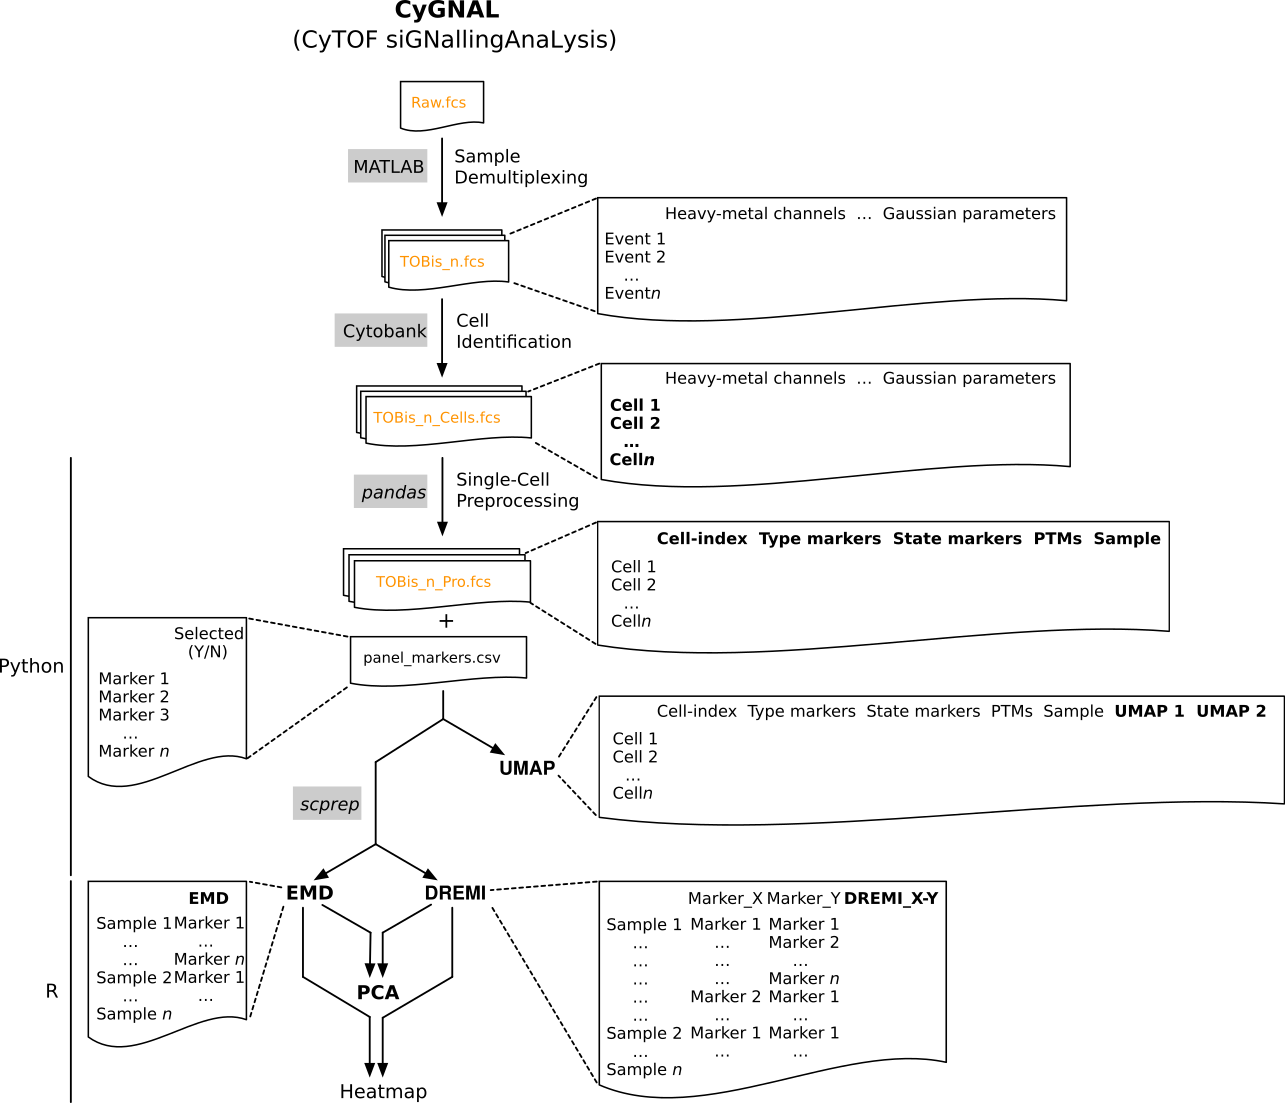
\includegraphics{03cytof/figs/3CYGNAL_pipeline.png}
    \caption{PIPELINE CYGNAL. WIP, consider merging with the use case figure as the overlap is significant.}
    \label{fig:3cygpipe}
\end{figure}

A general overview of CyGNAL's structure is shown in Figure \ref{fig:3cygpipe}, where the tool encompasses the bottom two thirds of the diagram.

As CyGNAL uses FCS files or tab-separated plain text files, certain upstream processes are necessary after data acquisition. Previous to analysing the data in CyGNAL, the standard operating procedure in our lab is to debarcode the mass cytometry datasets in MATLAB (using the tool from \href{github.com/zunderlab/single-cell-debarcoder}{github.com/zunderlab/single-cell-debarcoder}) and perform initial data pre-processing and quality control in Cytobank (\href{www.cytobank.org}{www.cytobank.org}). In that platform, the single cells are gated for Gaussian parameters, their DNA content, and uptake of Cisplatin using manual gates. Gating on cell state and cell type specific markers can also be done in order to both eliminate doublets but also to identify cells belonging to each state or type; information which can then be used to understand the biological system, but also train the cell state classifier.

CyGNAL proper starts with the pre-processing step. Here, empty heavy metal channels with no conjugated antibodies are removed, and the remaining channels are renamed to reduce the presence of special characters and keep with the naming conventions of the Fluidigm CyTOF software. A unique cell identifier is also given to each cell, and experimental metadata can also be embedded within the main pandas dataframe. Furthermore, a file with update antibody channel names is also saved (panel\_markers.csv), so that the user can select which channels to use in downstream steps.

Dimensionality reduction via Uniform Manifold Approximation and Projection (UMAP) \cite{mcinnes_umap_2020} can be performed to embed the individual cells on a 2-dimensional space based on the select antibodies.

EMD and DREMI scores are computed using the scprep package \cite{noauthor_krishnaswamylabscprep_2021}. Compute time can be reduced by subsetting the panel to channels of interest, and the user gets prompted to define specific arguments relevant to either computation, such as defining the variable and reference distributions for the EMD step.

Finally, the computed EMD and DREMI scores can be visualised as heatmaps or further summarised via PCA to compare profiles across conditions using CyGNALs last two main steps. The visualisation steps load in the default and user-given parameters and pass them to R Shiny-Apps \cite{noauthor_rstudioshiny_2021} that host a local server which automatically opens on the browser.

\subsection{Use Case and Outputs}

CyGNAL is distributed with sample mass cytometry datasets, which originate from technical replicates of an organoid monoculture experiment. They have been downsampled so that they can be hosted on GitHub and distributed with the code itself. The results presented in Figure \ref{fig:3cygvis} A-C were generated with this sample data.

In Figure \ref{fig:3cyguse} I present a mass cytometry dataset from Qin \emph{et al.}~\cite{qin_cell-type-specific_2020} to showcase an example use with heterotypic culture conditions where cell type specific analysis is necessary. The data belongs to the same mouse colon organoid model from Chapter \ref{04seq} and presents with a similar experimental setup, wherein organoids with different genotypes where cultured on their own or with macrophages and/or fibroblast cells. Data was subsequently gated and annotated on cell types and states as described above and on the original publication \cite{qin_cell-type-specific_2020}, and then passed onto CyGNAL for preprocessing (Figure \ref{fig:3cyguse} A).

\begin{figure}
    \centering
    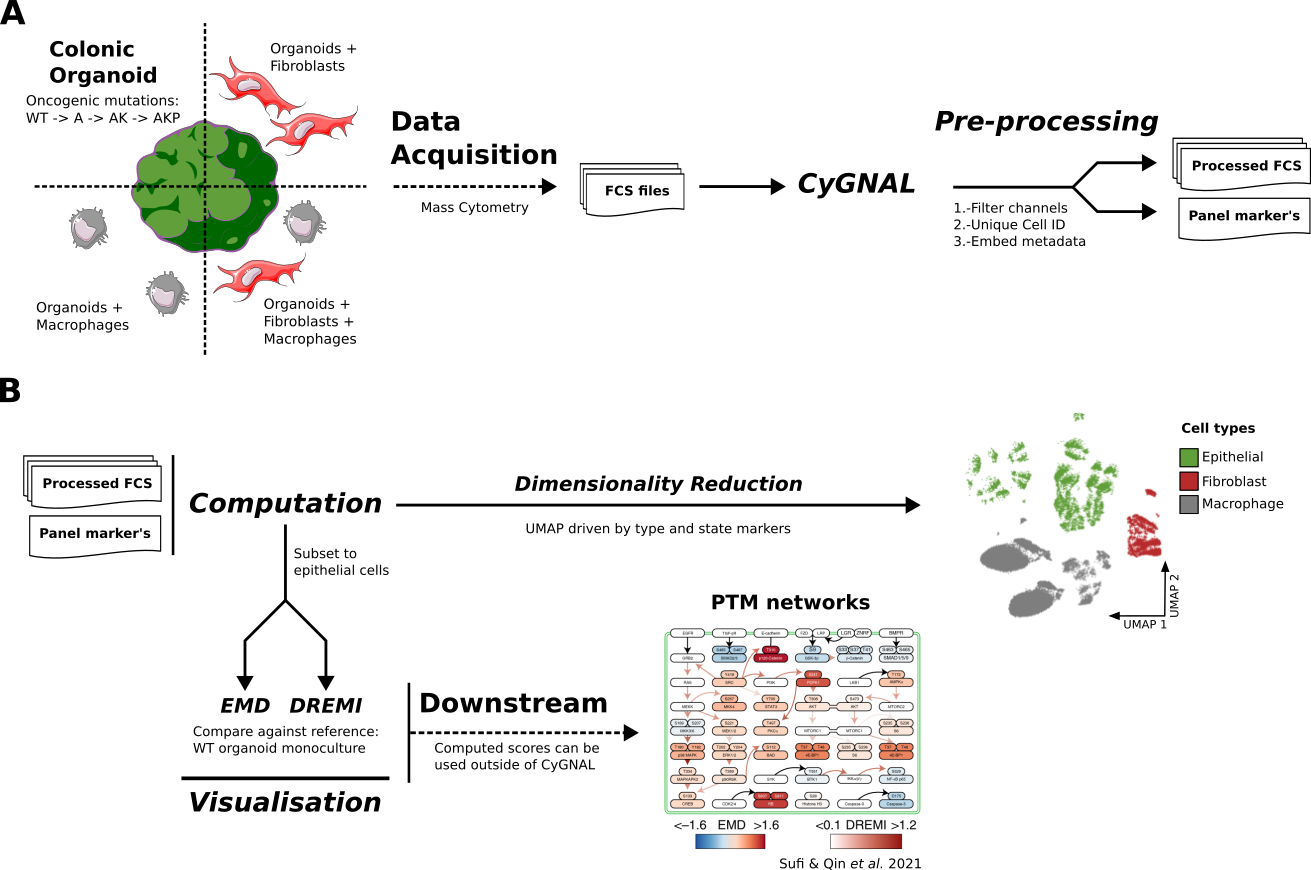
\includegraphics{03cytof/figs/3CYGNAL_usage.png}
    \caption{}
    \label{fig:3cyguse}
\end{figure}

Cell state and type markers were then selected from the panel marker file (pHH3, IdU, cCasp3, pRB, LRIG1, CEACAM1, pan-CK, F4/80, PDPN, RFP, CyclinB1, CD68) from which the UMAP embedding was generated (Figure \ref{fig:3cyguse}B). Embedding resolves the three distinct types (Figure \ref{fig:3cyguse} B).

Using the cell-type gates previously drawn on Cytobank, unique cell identifiers were used to select only the organoid cells. Computation of EMD and DREMI scores was then performed on the epithelial compartment, and can be visualised as part of CyGNAl. Furthermore, in the specific context of PTM network signalling analysis, EMD and DREMI scores can be used to assemble signalling network diagrams. With EMD used to quantify PTM node intensity and DREMI to score PTM-PTM edge connectivity, a signalling network can be curated and manually annotated as shown in Qin \textit{et al}. 2020 \cite{qin_cell-type-specific_2020}. 

When paired with a well-curated antibody panel and robust experimental design, TOBis MC allows multiplexed analysis of cell type–specific PTM signalling of heterocellular organoids \cite{sufi_multiplexed_2021}. 

\begin{figure}
    \centering
    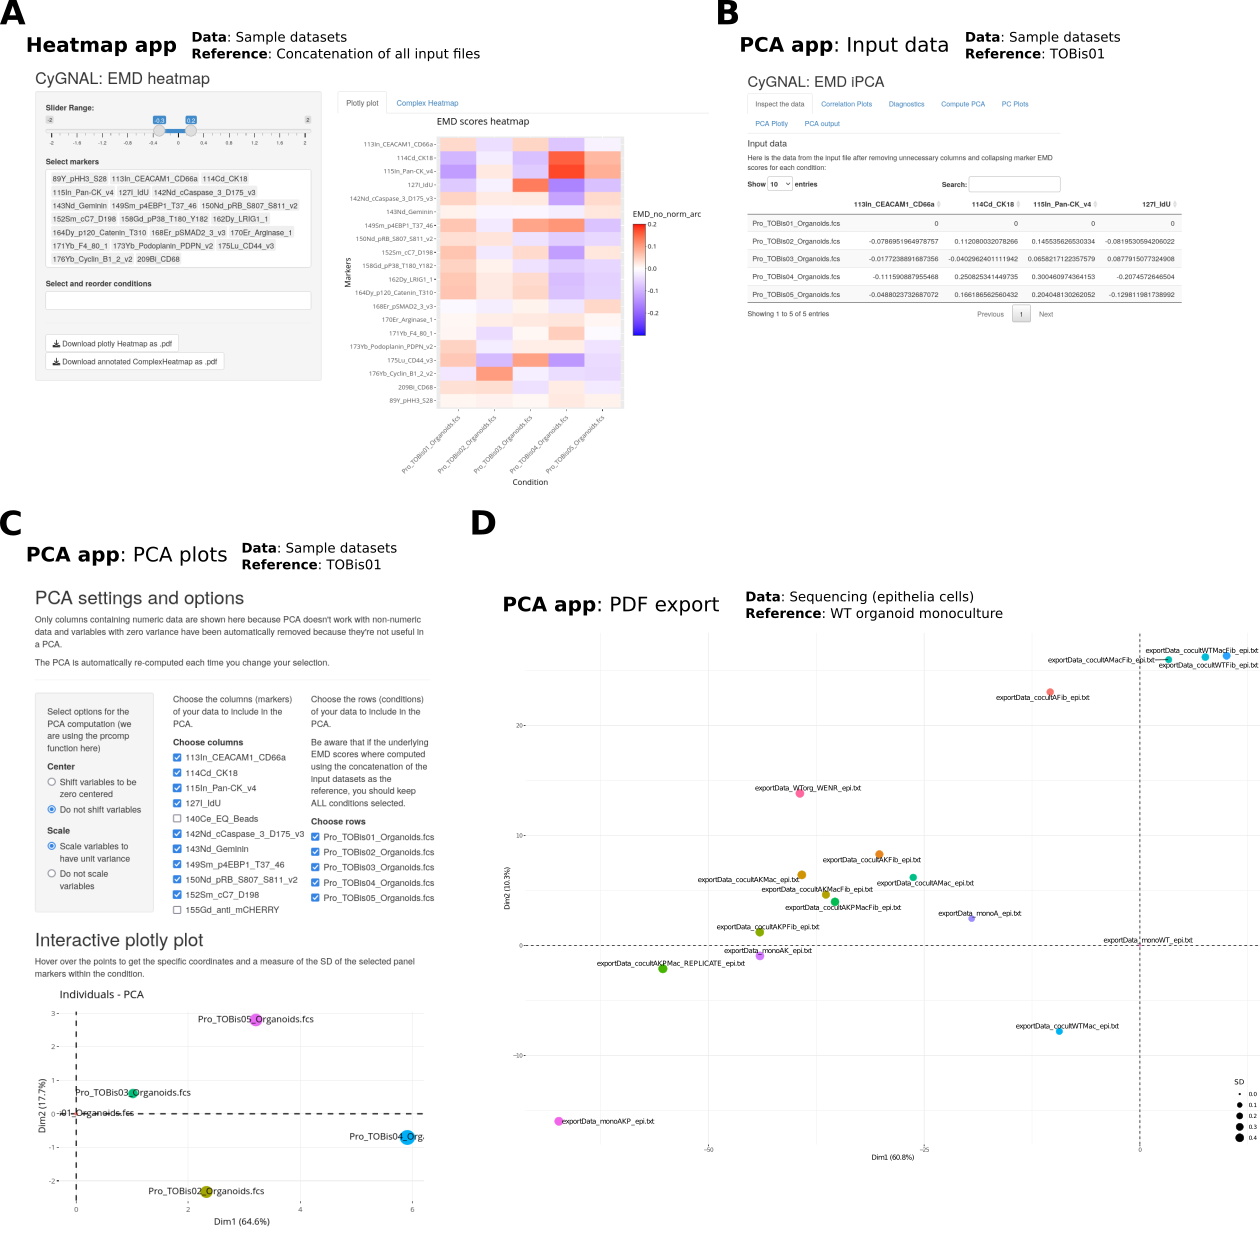
\includegraphics{03cytof/figs/3CYGNAL_usageVIS.png}
    \caption{Manual gates vs Tree vs Forest}
    \label{fig:3cygvis}
\end{figure}

Using the sample data and with the concatenation of all input files as the reference for the EMD step, Figure \ref{fig:3cygvis}A demonstrates CyGNAL's heatmap visualisation. By selecting not to use a specific reference during the EMD computation step, the generated scores are useful to compare how antibody expression compares across each of the individual datasets/conditions. The heatmap ShinyApp lets the user control the colour scale (automatically set to maximise contrast on the range of EMD scores), remove antibodies from the heatmap, and reorder the datasets/conditions shown in the columns. The heatmap shown in Figure \ref{fig:3cygvis}A is an interactive version generated with Plotly \cite{plotly_technologies_inc_collaborative_2015}, and shows the corresponding EMD score when hovering over a cell. Furthermore, a similar non-interactive heatmap is generated using the ComplexHeatmap \cite{gu_complexheatmap_2021} package and can be found within its homonymous Shiny-App tab.

The same data was used when running the PCA Shiny-App in Figure \ref{fig:3cygvis}B-C. This CyGNAL steps lets the user explore the data by looking at the raw scores (Figure \ref{fig:3cygvis}B) and Pearson correlation between channels. The user can also define parameters for the Principal Components Analysis, including the number of markers, generate several types of PCA plots with or without eigenvectors overlaid, and export the PCA results as plain text. In Figure \ref{fig:3cygvis}D I demonstrate how, despite CyGNAL being originally designed to handle mass cytometry data, other types of single-cell omic data like scRNA-seq can also be used. Here I used CyGNAl to compute EMD scores based on the gene expression of the organoids sequenced in Chapter \ref{04seq} and generate a PCA embedding showing how the different conditions compared to the control.
Note that the PCA data in Figure \ref{fig:3cygvis}B-D was generated using EMD scores computed with a particular dataset/condition as the reference and without centring the PCA embedding matrix, exemplifying use cases where we have a clear control condition against with the other conditions are compared (like the WT organoid monoculture in Figure \ref{fig:3cygvis}D).

\newpage
\section{Cell-state Random Forest Classifier}

\begin{figure}
    \centering
    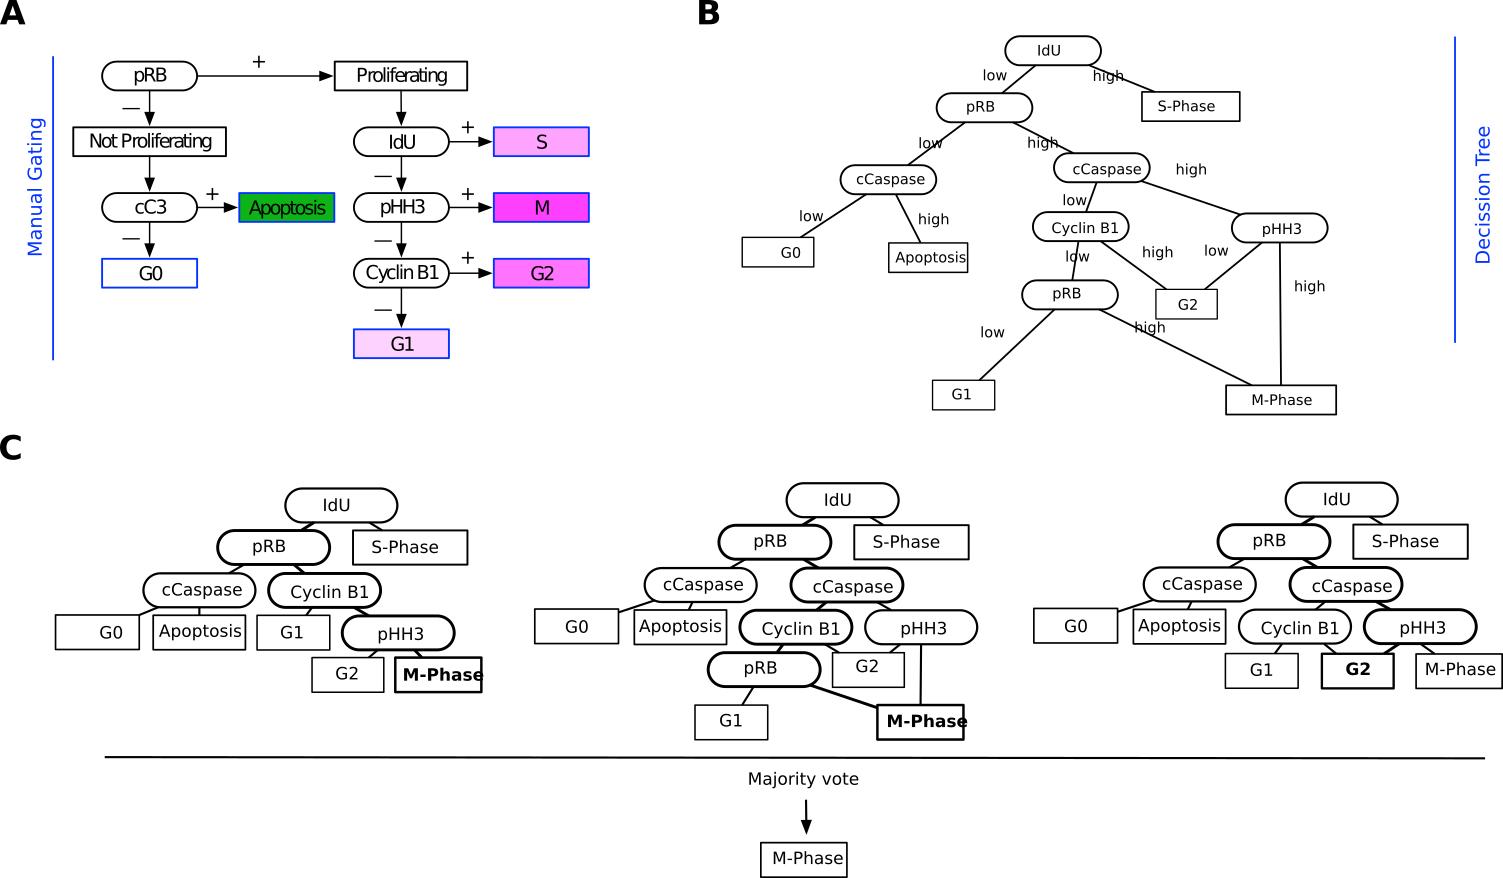
\includegraphics{03cytof/figs/3CLASS_stateRF.png}
    \caption{FINISH THIS FIGURE AND CHANGE COLORS TO MATCH METHODS}
    \label{fig:3classover}
\end{figure}

Determining a cell's state with regards to the cell-cycle phases is central to understanding the intestinal epithelium response to perturbations, as shown by Qin et \emph{al.} and their observations regarding cell-type specific regulation of cell states in response to microenvironmental and oncogenic cues~\cite{qin_cell-type-specific_2020}.

The cell states labels are commonly established using manual gating on a biaxial marker state, wherein a researches draws a boundary separating 2 groups of cells, essentially thresholding the data based on antibody expression. While strategies differ widely, a common approach taken by my lab is depicted in Figure \ref{fig:3classover}A. However, generating these cell state labels is a time consuming process, especially when compounded with the scalability of \acrshort{mc} and TOB\emph{is} ability to perform highly multiplexed analyses. Issues with user-induced biases are also present, as drawing the manual gates is a subjective process that might not remain consistent from experiment to experiment.

Early on my PhD I was exploring the link between \acrshort{ptm}s and cell state when I noticed that the process of generating the cell state labels could potentially be automated using a classical supervised machine learning approach. Eventually thus, I developed a cell state \acrlong{rf} (\acrshort{rf}) classifier to automate this process (see Chapter \ref{02methods} for more details). The manual gating process naturally resembles the logic behind a decision tree, for in both a threshold of antibody intensity would result in a binary classification of cell groups (Figure \ref{fig:3classover}A-B). Furthermore, the \acrshort{rf} machine learning approach remains a white box whose internal decision logic can be easily interpreted, for it consists of a collection of individual decision trees trained on subsets of the data that are used together in an ensemble approach (Figure \ref{fig:3classover}).

\subsection{5-marker model performs across model systems}

\begin{figure}
    \centering
    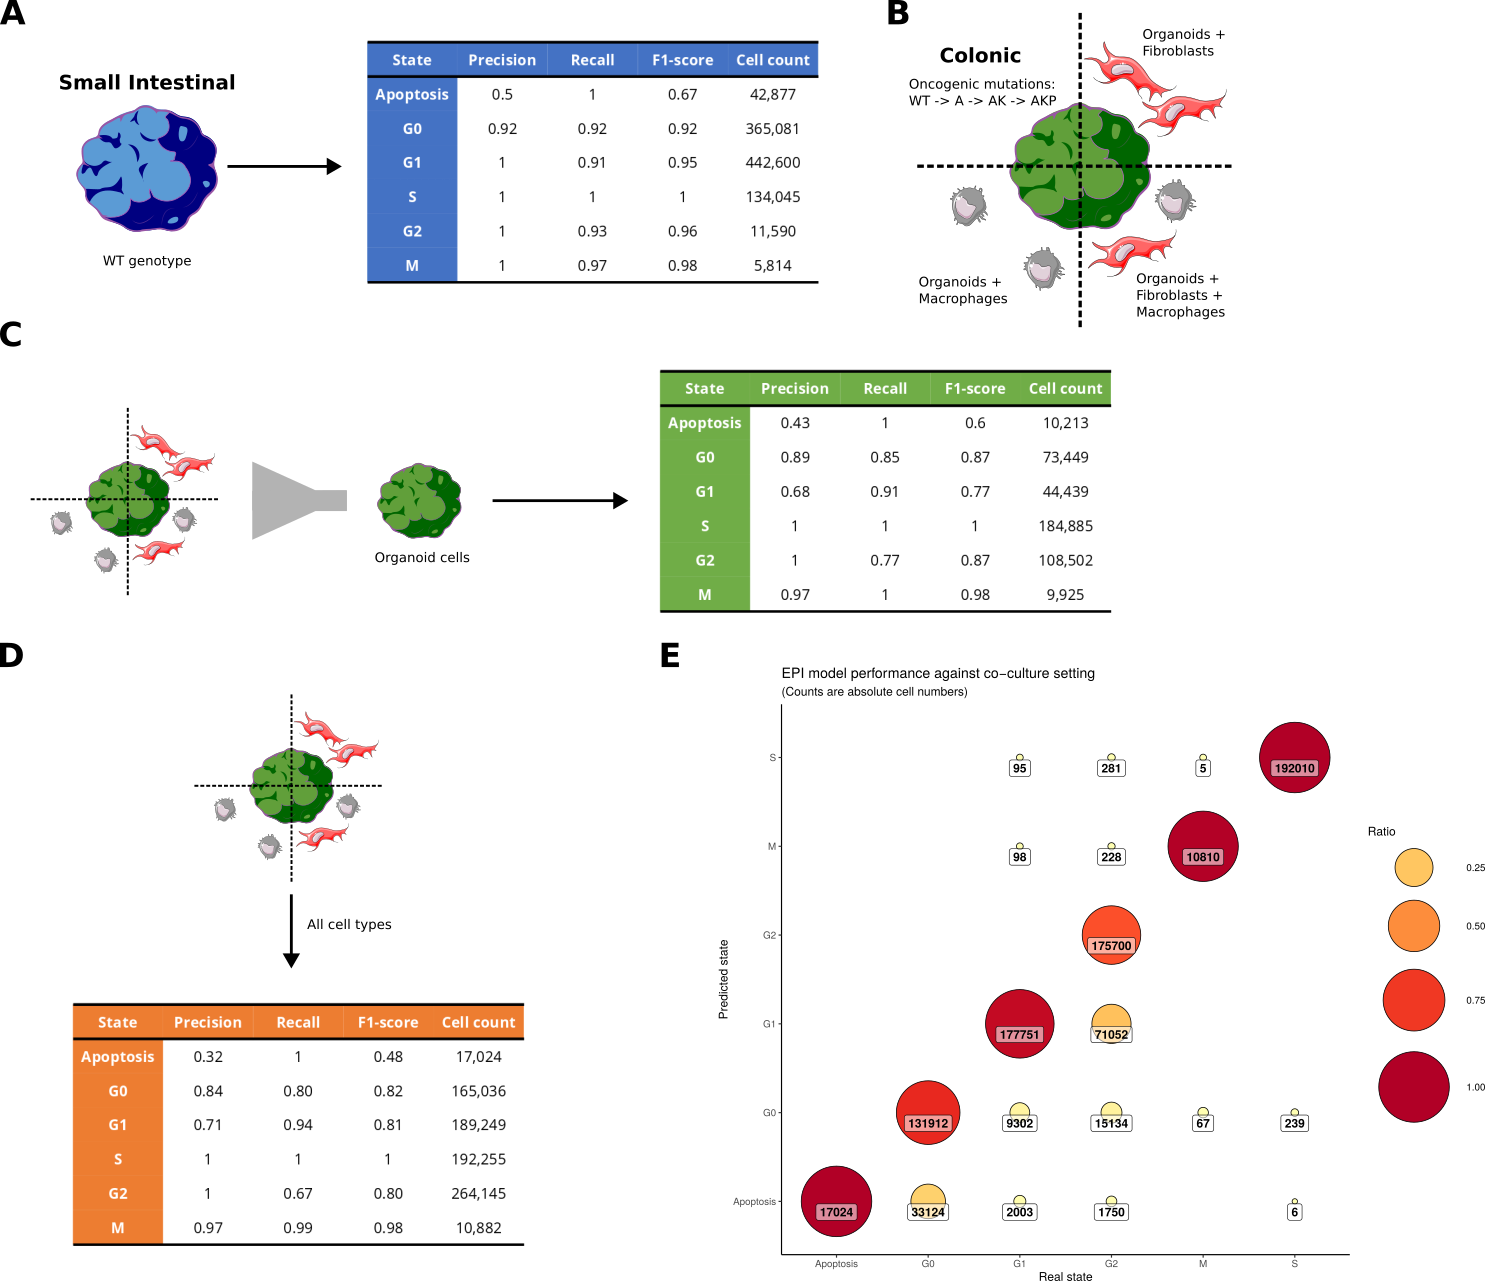
\includegraphics{03cytof/figs/3CLASS_5m.png}
    \caption{Benchmarking 5-marker RF cell state classifier. Shown in a), b), and c) are the classification reports obtained from running the 5-marker RF classifier against data manually labelled for cell state (representing the “real state” or ground truth). In a) a single timepoint SI LGR5 dataset was used, very similar to the training data for the model. The dataset in both b) and c) is a coculture of CRC organoids and their TME, with the cells in b) being a subset of the whole dataset containing just epithelial cells. Decreasing levels of performance correlate with increasing differences between the train and test datasets, as can be seen by the low f1-scores for the apoptotic class in c). Using the same data as c), the dot plot derived from the classification matrix in d) depicts the number and proportion (as both size and colour of the circles) of mislabelled cells for each cell state, showing that a considerable number of falsely mislabelled apoptotic cells are actually in G0 phase and some cells. RF: Random Forest.}
    \label{fig:3class5m}
\end{figure}

The first \acrshort{rf} model built was trained on data from the murine small intestinal organoid cultures from Qin et \emph{al.}~\cite{qin_cell-type-specific_2020}, consisting of \acrshort{wt} organoids along several developmental time points (Figure \ref{fig:3class5m}A). This model used only the 5 markers shown in Figure \ref{fig:3classover}A. Details on building the model and the relative feature importance when training can be found in Chapter \ref{02methods}.

Testing the 5-marker RF model on a different single time-point small intestinal organoid dataset also from Qin \textit{et al}. \cite{qin_cell-type-specific_2020} results in global accuracy for all classes of 0.93. However, $F_1$ scores reveal a big performance drop with the apoptotic class (Figure \ref{fig:3class5m}), driven by the low 0.5 precision score when predicting the apoptotic label. Precision scores otherwise remain above 0.92 for the other labels.

Performance of the classifier drops when testing against the CRC TME colonic organoid cultures from Qin \textit{et al}. \cite{qin_cell-type-specific_2020}. In this case, subsetting just the organoid cells from the organoid cultures (Figure \ref{fig:3class5m}B), we observe a global accuracy of 0.91. Looking at the classification details (Figure \ref{fig:3class5m}C) we see a very similar pattern to the SI LGR5 results; with the apoptotic class presenting the lowest $F_1$-scores (0.6) characterised by a low precision (0.43). Furthermore, the remaining $F_1$-scores are also lower overall, with only the S-phase and M-phase classes reaching above 0.9.

When no epithelial filter is applied to the dataset and the model performance is tested against all cell types (i.e., including also fibroblasts and macrophages) global accuracy drops down to 0.87. The relatively high global accuracy does not reflect the failure of the classifier to, yet again, identify the apoptotic cells (Figure \ref{fig:3class5m}D). In Figure \ref{fig:3class5m}E the classification matrix is used to build a dot plot in which the true labels (“Real state” from gating) are compared against the predicted labels (“Predicted state”), highlighting how a majority of the cells labelled as apoptotic are actually G0 cells, explaining the precision of 0.32 for the former class. There is also some confusion around the G2 cells, as a significant number of these cells are classified as either G0 or G1.

\subsection{10-marker model improves apoptotic classification}

\begin{figure}
    \centering
    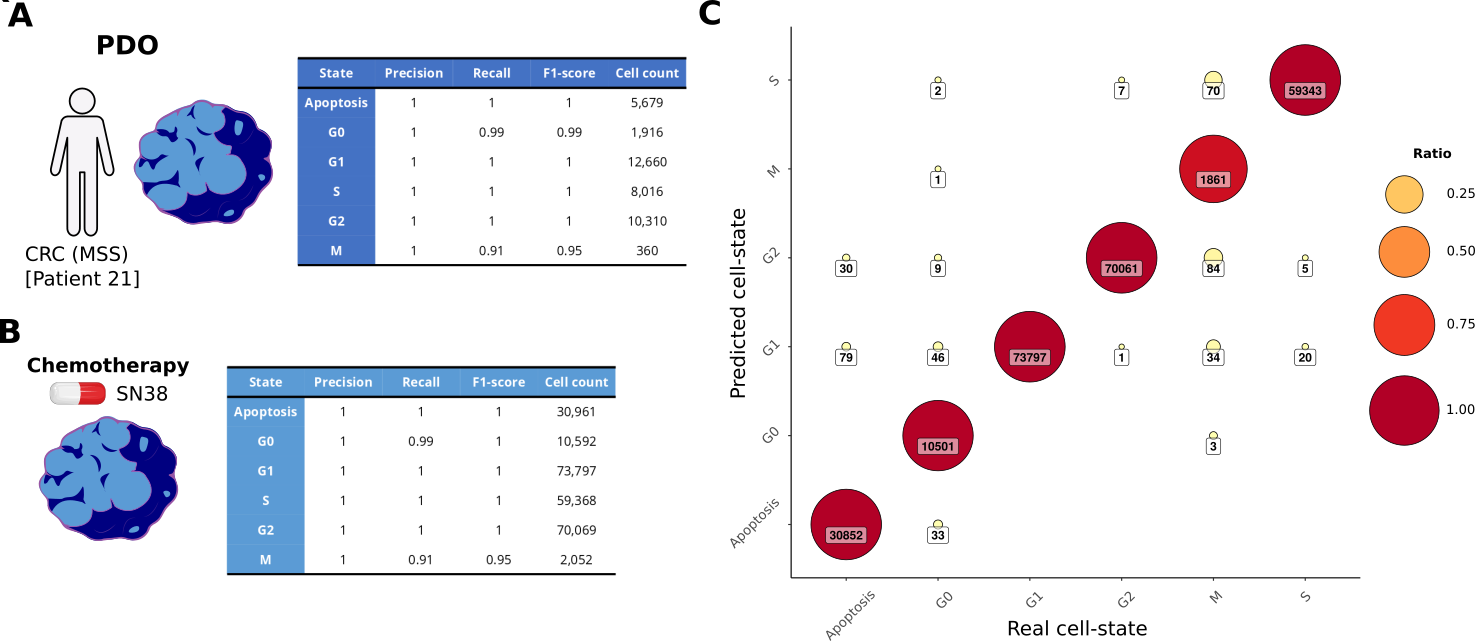
\includegraphics{03cytof/figs/3CLASS_10m.png}
    \caption{Benchmarking the new 10-marker RF cell state classifier. Building a RF classifier with an increased number of markers using data from PDOs renders better results than the original 5-marker model, as can be seen in a) with the classification report. b) Classification matrix generated automatically during model building, showing extremely low levels of misclassified cells. RF: Random Forest. PDO: Patient-Derived Organoids. Labels: 0=Apoptosis, 1=G0, 2=G1, 3=S-phase, 4=G2, 5=M-phase.}
    \label{fig:3class10m}
\end{figure}

Given the 5-marker model limitations when resolving the apoptotic class, I implemented a second model using additional \acrshort{ptm} antibodies and cell state markers targeting apoptotic cells. This 10-marker model uses a dataset from Zapatero \& Tong \emph{et al.}~\cite{zapatero_trellis_2023} wherein heterotypic \acrlong{pdo} (\acrshort{pdo}) cultures from different donors were treated with a spectrum of chemotherapies. This data was generously provided by Dr. Maria Ramos Zapatero.

Results from the updated 10-marker implementation using \acrshort{pdo} data show improved performance when compared to the 5-marker model. Using a technical replicates of the training data as test we observe how the apoptotic class gets accurately resolved (Figure \ref{fig:3class10m}A). When benchmarking the model performance against a dataset wherein the organoid cells had been treated with SN-38, the active metabolite of the type I topoisomerase inhibitor Irinotecan \cite{mathijssen_clinical_2001}, we observe a global accuracy greater than 0.99. The lowest $F_1$-scores, at 0.95, were found for the M-phase label (Figure \ref{fig:3class10m}B). This lowered, yet still accurate, prediction performance is driven by the lower total count of M-phase cells (one order of magnitude smaller than the other classes), hampering the training for that class and resulting in small number of non-apoptotic cells to be miss-labeled as M-phase.
In contrast with the 5-marker model results, there is an apparent lack of issues when classifying the apoptotic class, with only 0.35\% of true apoptotic cells being mislabelled (Figure \ref{fig:3class10m}).

\newpage
\section{Conclusions}

In this chapter I have shown how CyGNAL is an accessible workflow to non-computational users that facilitates data processing and analysis of \acrshort{mc} experiments. The computation of \acrshort{emd} and \acrshort{dremi} scores enables a detailed mechanistic description of changes across conditions, wherein changes in the user defined reference allows for differential interrogation of the experimental system. 

While the scores themselves can be used to build curated mechanistic models as in Qin \emph{et al.} \cite{qin_cell-type-specific_2020}, CyGNAL also incorporates interactive visualisation modules that can automatically plot results. The interactive nature of the visualisation steps, coupled with additional data correlation metrics given during the \acrshort{pca} computation, allows for both exploratory data analysis and (close to) publication grade results generation within a single tool. This same \acrshort{pca} computation presents a straightforward way to summarise changes at the condition level from otherwise information-dense \acrshort{emd} or \acrshort{dremi} heatmaps.

The incorporation of miscellaneous data handling helper scripts in the utilities folder exemplifies how user-provided feedback is paramount, while it also signifies how CyGNAL continuously grows and changes with time. Tools are meant to be used, and that publications by colleagues such as Michelozzi \emph{et al.}~\cite{michelozzi_activation_2023} employed CyGNAL is a testament to its accessibility.

Originally meant as a simple exercise in curiosity-driven exploration after noticing the correlation between so called PTM and "cell state" markers, and empowered by the tediousness of manually gating the datasets in our lab, the \acrshort{rf} cell-state classifier has become a convenient tool to automate cell-state labelling of \acrshort{mc} datasets in relation to cell-cycle phases.

Albeit a very simple model, the nature of the manual gating process (essentially thresholding on a biaxial space of marker expression) translates well to decision trees, and this is shown in the relatively strong overall model performance. The current implementation however, might struggle to generalise to external datasets, for gating strategies are somewhat of a lab- and individual-specific process.

Where we do observe weak points in the classifier is for those cell state labels whose antibody coverage is not great in the model. For example, in the 5-marker \acrshort{rf} model, apoptotic cell class precision reaches only 0.32 in the most stringent setting tested (Figure \ref{fig:3class5m}D). This can be relatively straightforward to address by increasing the number of antibodies targeting that particular state (Figure \ref{fig:3class10m}B-C), but this strategy can not always be employed as the additional marker would both need to be in the reference data used to train the model and in the query dataset to be labelled. When possible however, as demonstrated by the the 10-marker \acrshort{rf} model built, high precision and recall scores are accomplished for all cell states even in the context of cell-cycle disrupting chemotherapy (Figure \ref{fig:3class10m}B-C).

As described in Chapter \ref{02methods}, both tools are publicly accessible in their respective GitHub repositories. 